%%% $Id$
%%% Copyright (C) 2002 Greg J. Badros <greg.badros@infospace.com>
%%
%
% This file should be compiled with V1.0 of "www2003-submission.cls"
%
% ----------------------------------------------------------------------------------------------------------------
% This .tex file (and associated .cls V1.0) produces:
%       1) NO Permission Statement
%       2) WWW'03-specific conference (location) information
%       3) The Copyright Line with ACM data
%       4) NO page numbers
%
% ---------------------------------------------------------------------------------------------------------------
% This .tex source is an example which *does* use
% the .bib file (from which the .bbl file % is produced).
% REMEMBER HOWEVER: After having produced the .bbl file,
% and prior to final submission, you *NEED* to 'insert'
% your .bbl file into your source .tex file so as to provide
% ONE 'self-contained' source file.
%

\documentclass{www2003-submission}
\usepackage{times}
\usepackage{moreverb}
\usepackage{floatflt}
\usepackage{url}

\newcommand{\B}{\discretionary{}{}{}}
\newcommand{\smtt}{\small}
\newcommand{\smtexttt}[1]{{\small\texttt{#1}}}
\newcommand{\ns}[1]{{\small\texttt{#1:*}}}
\newcommand{\figref}[1]{Fig.~\ref{fig-#1}}
\newcommand{\secref}[1]{Section~\ref{sec-#1}}
\newcommand{\ssecref}[1]{Section~\ref{ssec-#1}}
\newcommand{\tableref}[1]{Table~\ref{#1}}
\newcommand{\tm}{{\scriptsize $^{\mbox{tm}}$}}
\newcommand{\gjb}[1]{{\sc gjb:}\textbf{#1}}

\begin{document}
%
\title{The Extensible Templating Language: \\
       Improving Analysis of Markup Generating Code}

\numberofauthors{1}

\author{
%
% The command \alignauthor (no curly braces needed) should
% precede each author name, affiliation/snail-mail address and
% e-mail address. Additionally, tag each line of
% affiliation/address with \affaddr, and tag the
%% e-mail address with \email.
\alignauthor Greg J. Badros\\
       \affaddr{InfoSpace, Inc., 601 108th Ave. NE, Suite 1200, Bellevue, WA 98004, USA}\\
       \email{greg.badros@infospace.com}
}
\date{12 November 2002}
\maketitle
\begin{abstract}
ETL.... \gjb{Write this!}

\end{abstract}

% A category with only the three required fields
%% GREGB:FIXME::
%% See http://www.acm.org/class/1998/overview.html
\category{D.2}{Software}{Software Engineering}
\category{D.3}{Software}{Programming Languages}

% GREGB:FIXME:: any terms?
%\terms{}

\keywords{Restricted domain-specific programming language, static analysis,
web server, templates, XML, XSLT, markup, WML, HTML.}

\section{Introduction}
\label{sec-intro}

The loosely-coupled client/\B{}server model implied by the current
breed of applications deployed via the World Wide Web presents
substantial new complexities for application developers. A variety of
new programming languages and paradigms attempt to address these novel
problems.  One important characteristic of this new world of software
development is the need to generate HTML, WML, or other markup
languages to describe client-side presentation and behaviour.

The original server-side dynamic markup-generation capabilities of the
Web were defined by the Common Gateway Interface.\cite{CGI11} For each
request of a CGI, the web server maps HTTP request details into environment
variables, command-line arguments, and the standard file descriptors.
In particular, the standard output written by that process was sent by
the Web server as the response to the client browser (instead of
simply responding with an unchanging file from disk).  Over time,
various techniques arose to reduce the cost of each request: extension
mechanisms such as the Apache module system~\cite{Apache} and
scripting languages hosted by the Web server have increased
performance by eliminating process creation overhead.

Today, server-side markup generation is dominated by expressive and
flexible general-purpose programming languages such as
Java~\cite{Arnold98}, Perl~\cite{Camel3rd}, and PHP~\cite{pro_php}.  Ironically,
the languages are then used in fairly restricted ways, often being
tied to a templating syntax (e.g., JSP~\cite{JSP12} for Java or
HTML::Template~\cite{HTML-Template} or Mason~\cite{Perl-Mason} for Perl).  For example, consider
the PHP template in \figref{php-books}.  The only constructs required
by the template are a) some means of populating a data model from the
back-end business logic (line 1); b) data-driven iteration (line 4-5);
and c) simple expression evaluation to access parts of the data model
(lines 7 and 9). % GREGB:FIXME:: check these line numbers The extra
power provided by typical templating languages not only goes unused,
but it also complicates certain important analyses of the code.  For
example, the obviously important property that a template execution
terminates is undecidable for these general purpose languages.

\begin{figure}[tb]
\begin{listing}{1}
<? $books = GetBooks(...); ?>
<html>
 <table>
  <? for ($i = 0; 
           $i < count($books); ++$i) { ?>
   <tr>
     <td><? print($books[$i][author]); ?>
         </td>
     <td><? print($books[$i][title]); ?>
         </td>
   </tr>
  <? } ?>
 </table>
</htm>
\end{listing}%$
\caption{PHP template illustrating the simplicity of the programming
language constructs required by typical templates.  Unfortunately,
because a powerful language is provided, PHP templates often engage in
far broader interactions than the above ideal example.
\label{fig-php-books}}
\end{figure}

Unfortunately, for most contemporary web application development
frameworks, the restrictions desired of the front-end templating layer
are imposed only by process and convention.  Template authors are
asked to limit themselves to a subset of the available features of a
language as a means of facilitating scalable, secure, well-behaved
systems.  Importantly, however, there is nothing inherent that
prevents template-based code from, for example, making individual
database connections (which would impact performance) or maintaining
undesirable server-side state (which would impose additional
requirements on the load-balancing mechanism and reduce scalability).
These concerns are intensified because many development organizations
encourage a strong separation between the web developers and back-end
application developers. While web developers have substantial
expertise in HTML, user-interface design, and client-side scripting,
their responsibilities often do not include consideration of the
larger architecture.

Another substantial problem with existing templating technologies is
that they often involve the lexical mixing of two separate programming
paradigms.  JSP, for example, is implemented in terms of a
pre-processing rewrite of the template into a Java servlet.~\cite{JavaServlet23}
Pre-processing approaches are convenient for programmer expressiveness
but have a huge hidden cost in complicating software engineering
analyses and tools that would otherwise help understand, maintain, and
evolve the complex systems~\cite{Badros00-spe,ErnstBadrosNotkin02}\cite[p.~424]{Stroustrup94}.
The precise analysis of an arbitrary JSP template necessarily requires
full knowledge of both the rewrite rules and the semantics of Java.

\gjb{Stress spaghetti code, separation of front and back end, describe
how web service adoption changes the picture (reference the figure)}

\gjb{Any references for importance of separation of front and back end?}

\gjb{Question one assumption: do we need a full-blown general purpose
programming language?}

%% GIVE EXAMPLES OF VALUABLE ANALYSES!!!
\subsection{Analysis of markup templates}

The various templating languages all have one primary goal: to
generate markup to be returned to the requesting user agent.  It is
important that the markup created conforms to appropriate Internet
standards.  For example, WML markup needs to first be well-formed XML
and second be valid with respect to the appropriate
schema or DTD~\cite{WML12}.  Although HTML browsers are more forgiving of
variations in syntax, best-practices still dictate that the markup returned
be in compliance with the HTML specification~\cite{HTML4}.
Popular templating languages including PHP, JSP, ASP, and others
all process arbitrary text and are ignorant of the rules of the markup
being generated: the mistaken close tag on line 14 of \figref{php-books}
goes unnoticed by PHP.

Tools such as HTMLTidy~\cite{HTMLTidy} are available to check the
responses from servers for conformance, but often testing involves
simply using various browsers to exercise the application while
looking for bugs.  Both of these approaches require exhaustively
visiting every page of interest--often a very large search space.
Ideally, we would prefer a way to statically analyze the source templates
themselves to gain confidence that they will, in fact, generate proper
markup.  If static analysis of templates can rule out the possibility
of certain kinds of errors, testing time and costs can be dramatically
reduced.

Another important requirement for software development systems is to
support ad-hoc queries of the source code. For small and simple
dynamic web applications, the automated analysis of templates is often
unnecessary: a web developer or two understands all of the code.  Over
time, however, these simple applications grow in size and complexity
such that tools analyzing the templates become an essential part of
maintaining and evolving the system. For example, a site may wish to
add an extra input field to all of its registration forms.  If a
generic form is not already factored out into a common location, the
first step in approaching the task is finding all of the registration
forms.  Or suppose a new handheld device has a limitation in its
handling of cookies: we need a means of narrowing the scope of careful
review to places where that cookie is manipulated.

Typically, web developers approach to above scenarios with an arsenal
of imprecise lexical tools such as \smtexttt{grep}.  While searching
for a substring or regular expression may satisfy some simple queries,
when the desired query has additional structure, lexical approaches
fall short.  Suppose we wish to find dead code to simplify our
application. No regular expression will let us identify all
unreachable templates to satisfy that query.  To analyze more deeply,
we need to uncover the semantic structure of the templating language.
Typically, that requires a language-specific parsing approach and much
greater effort in building a valuable tool or an extensible integrated
development environment~\cite{Soroker97,Eclipse}.

\subsection{XML supports analyses and tools}

An increasingly popular approach to performing structured queries of
programming language source code is to use standard XML tools such as
XSLT~\cite{XSLT} and XQuery~\cite{XQuery} to operate over a
complementary XML-based representation~\cite{Badros-www9,others}.
With a carefully-chosen XML representation, valuable semantics of the
code are immediately available to XPath expressions, thus facilitating
a broad class of source code tools.  However, for a general-purpose
programming language, XML is unwieldy for use as the primary
representation.  Instead, the conventional grammar-based language is
edited by humans and is only converted into XML for the tools to
leverage.

This research applies the benefits of an XML representation of source
code to the domain of restricted markup templating languages.
Importantly, web developers working with templating languages are
already writing markup directly, thus making it natural for them to
express the limited logic of their dynamic templates directly in
markup as well.  This observation eliminates the dual representation
problem that restricts the value of XML when applied to general
purpose programming language.  The approach also enables the use of
schema-aware XML editors to provide a rich development environment
with very little ETL-specific effort (see \secref{benefits}).

In this paper, I introduce the Extensible Templating Language.  From
one perspective, ETL is a 100\% XML-based templating language that
embeds programming language constructs directly in the XML
representation, intermingled with literal target-language markup.
Alternatively, we can view ETL as an imperative domain-specific
programming language that uses XML as its surface syntax and
simplifies the writing of programs that generate markup languages.

ETL leverages the well-formedness and local-validity checks of the
source template to support those same properties in the generated
response markup.  By limiting the programming-language constructs to
include only the features that are appropriate at the front-end of a
scalable web application architecture, we ease numerous analyses and
encourage proper separation of the presentation from the content and
business logic. Finally, because of its use of XML as a
representation, ETL simplifies ad-hoc software engineering analyses to
better support evolution and maintenance of large dynamic web
applications.  We have built an ETL runtime inside of a
production-quality web server, the Extensible Templating Language
Server.  ETLS is currently employed by InfoSpace to serve over forty
million requests per day using over sixty thousand ETL templates.

\begin{figure}[bt]
\begin{centering}
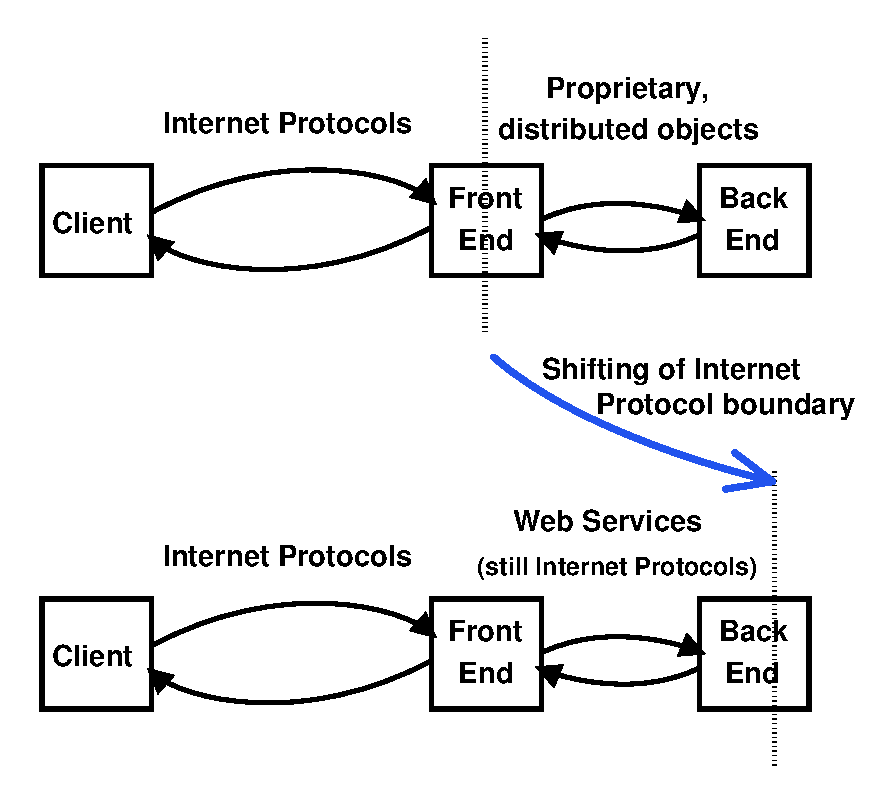
\includegraphics[width=1\linewidth]{web-service-ip-shift.eps}
\caption{Web services enable the front-end templating tier to
communicate with back-end applications via standard Internet Protocols
such as XML and SOAP; they no longer need to be aware of distributed
object protocols such as DCOM or Corba.\label{fig-ws-ip-shift}}
\end{centering}
\end{figure}


\subsection{Outline of paper}

The rest of this paper is organized as follows. \secref{etl} describes
the Extensible Templating Language itself. \secref{benefits} gives
several practical examples of the benefits of using a pure XML
approach with a restricted programming language.
\secref{implementation} details our implementation and
describes our experiences in using ETL in production systems over the
last year.  Finally, \secref{related-work} describes and contrasts
related work and \secref{conclusion} concludes.

%%% 
%\section{Background}
%\label{sec-background}

%% JSP/XML
%% XSLT

%\subsection{Current templating strategies}

%\subsection{Comparison of approaches}

%\begin{table}
%\centering
%\caption{Summary of existing templating approaches.}
%\begin{tabular}{|c|c|l|} \hline
%\\ \hline
%\hline\end{tabular}
%\end{table}


%%% 
%% GREGB:VISUAL:: avoid too obvious of an overfull hbox below
\section{\hspace*{-.1in}Extensible Templating Language}
\label{sec-etl}

The Extensible Templating Language is an imperative markup templating
language that allows web developers to intermingle literal XML markup
with XML-based programming language constructs.  Our primary design
goals for ETL were to:

\begin{enumerate}
\item Allow easy analyses of source templates to permit development of
supporting tools; 
\item support only the essential programming language constructs
required by a templating layer; and
\item utilize an XML data model pervasively to integrate seamlessly
with Internet and Web standards.
\end{enumerate}

An ETL template must be well-formed XML that is valid with respect to
several XML Schema Definitions.  The set of programming constructs
available in ETL is intentionally restricted to limit the amount of
logic performed in the front tier of a multi-tier web-delivered
application and better enforce proper separation of presentation from
content and business logic.  ETL is used by dozens of production
applications serving over forty million requests per day, thus
providing constructive evidence that the set of available constructs
is sufficient for real-world use.

\begin{figure}[tb]
\begin{listing}{1}
<?xml version="1.0"?>
<bl:template xmlns:bl="http://www....">
 <bl:set var="#xml/books">...</bl:set>
 <html>
  <table>
   <bl:for-each var="#xml/books/book">
    <tr> 
     <td><bl:get var="@author"/></td>
     <td><bl:get var="@title"/></td>
    </tr>
   </bl:for-each>
  </table>
 </html>
</bl:template>
\end{listing}%$
\caption{The ETL template corresponding to \figref{php-books}'s PHP
code. Because ETL is required to be well-formed XML, the developer
avoids the mistake from line 14 of the PHP example.
\label{fig-etl-books}}
\end{figure}

Because ETL is 100\% XML and because the language is not a full-blown
general purpose programming language, analyzing ETL templates for
various properties or searching for certain constructs is very well
supported.  In particular, because of the way literal markup is mixed
with programming constructs, the well-formedness requirement on the
source template greatly reduces the probability of common mistakes
including mismatching tags.  Additionally, we can also perform local
validity checks on literal markup elements to confirm their proper
nesting and that they use the correct attributes.  A goal of ETL is to
make approximate analyses easy and precise analyses possible.

An example ETL template appears in \figref{etl-books} and is analogous
to the PHP example from \figref{php-books}.  The program is simply an
XML document with root element \smtexttt{bl:template}\footnote{We use
namespace prefixes consistently to unambiguously refer to elements in
the distinguished namespace URIs recognized by the ETL server.}  The
template contains other elements in the \ns{bl} namespace which we
call ETL \emph{primitives} (see \ssecref{primitives}).  Additionally,
the template can contain markup from arbitrary other namespaces which
we call \emph{literal result markup} (see \ssecref{literal-markup}).

ETL templates are processed within the context of an HTTP request.
The path specified in the URL of the request is used to choose a
template from which processing begins (see
\ssecref{template-dispatch}).  URL and POST parameters, cookies, etc.,
are all available to the template (see
\ssecref{buckets}). The primary goal of executing a template is to
generate an HTTP response including the markup document along with the
various HTTP headers such as the content-type, cookie settings, and
other metadata.  Generally, an ETL template is similar to a method in
a general purpose object-oriented programming language: it can invoke
other templates as subroutines and can also perform subsidiary HTTP
requests to other servers.  In fact, HTTP-bound
web-service~\cite{WebServicesActivity} calls are the primary means of using
back-end application logic.

The remainder of this section informally describes the structure and
semantics of the Extensible Templating Language.


\subsection{Primitives, attributes, and slots}
\label{ssec-primitives}

An ETL primitive is an element in the \ns{bl} namespace that has a
specific well-defined behaviour inside of an ETL template.  Primitives
either output text to the current destination stream (initially the
response document) or perform some side-effect (or both).  For example
the \smtexttt{bl:set} primitive assigns a variable a value without
outputting any text, while the
\smtexttt{bl:http} primitive outputs either \smtexttt{http} or
\smtexttt{https} based on whether the current request arrived over an
ordinary or secure socket connection.

The behaviour of a primitive is parameterized by the various
attributes allowed on that element.  Some primitives, such as
\smtexttt{http} mentioned above, are always empty---they never are
allowed to contain child elements. 
Other primitives are allowed to be non-empty, using the markup generated
by their contained elements as an extra implicit argument.  For example,
in:

\smtexttt{<bl:if var="showcopyright"> (C) 2002 </bl:if>}

\noindent the contents of the \smtexttt{bl:if} are output if and
only if the variable is non-empty.

Many primitives derive their arguments not from individual attributes
but from pairs of attributes that are together called a \emph{slot}.  For
example, the \smtexttt{bl:cr} directive outputs linefeeds, and the
number of linefeeds it generates is determined by a slot called
\smtexttt{count}.  That slot is specified using a pair of attributes:
\smtexttt{count} and \smtexttt{count-var}.  The attributes are
mutually-exclusive: it is a statically-checked error to specify both on
the same \smtexttt{bl:cr} element.  The \smtexttt{count} attribute has
type \smtexttt{xsd:integer} and is used to provide a literal integer
argument to the primitive.  In contrast, the \smtexttt{count-var}
attribute has type \smtexttt{bl:identifierType} (a restriction of
\smtexttt{xsd:string}) and names a variable to evaluate at runtime to
determine the argument to the primitive.  In both cases, the integer
value of the argument is used as the number of linefeeds to generate,
but for \smtexttt{@count} that number is set statically while for
\smtexttt{@count-var} it is determined dynamically (at run-time).

Using a pair of attributes to represent a logical field is a novel
mechanism to improve the type-safety and ease analysis.  The common
alternative is using a small domain-specific language inside the value
of an attribute.  For example, we could have used \smtexttt{count="2"}
or \smtexttt{count="\$num"} to represent the literal number 2 or the
desire to use the current value of the variable ``num'',
respectively.\footnote{XSLT takes a similar approach, using, for example,
\smtexttt{value-of="'literal'"} or \smtexttt{value-of="var"} where the
value of the attribute is an XPath expression.}
Unfortunately, when using a single attribute, the type for the
attribute's value must be broadened and is hence less precise.
Additionally, developers must learn various ad-hoc syntactic rules to
ensure full-fidelity of values:  how do you express the literal string
``\$num'' when that sequence of characters means a reference to the
variable ``num''?  All analysis tools the become burdened with the
need to handle the case of, say, a backslashed ``\$'' character and
the rest of the quirks of the syntax.

Primitives can, of course, have numerous arguments, some of which are
controlled by slots and others by individual attributes.  When an
argument is allowed to be set only via an attribute instead of a slot,
that parameter of the directive cannot be influenced at
runtime---often this restriction is imposed to permit optimizations or
to improve our ability to support static analyses.  For example,
\smtexttt{bl:get} writes out the value of a variable and has a
\smtexttt{@transform} attribute that supports various encodings or
decodings of the value (e.g., \smtexttt{url-encode} or
\smtexttt{xml-decode}---see \ssecref{transformations}).  We disallow the
use of \smtexttt{@transform-var} because we want to always know from
static inspection what transformations may occur, thus facilitating
some analyses and optimizations.

\subsection{Variables and values}
\label{ssec-variables}

Variable values are set using \smtexttt{bl:set}.  Variables
declared in the header of a template are statically scoped to just
that template.   Undeclared variables are dynamically scoped until the
end of processing the current request.  A \smtexttt{bl:set} primitive
specifies the target variable as the \smtexttt{@var} attribute. The
value to be assigned is either given using \smtexttt{@value},
\smtexttt{@value-var}, or by executing the children of the
\smtexttt{bl:set} element.  For example:

\begin{verbatim}
<bl:set var="baseuri"><bl:http/>://<bl:get
 var="hostname"/>/</bl:set>
\end{verbatim}

\noindent might set the variable named ``baseuri'' to the value
``http://www.\B{}infospace.\B{}com'' (assuming the request comes as an
ordinary insecure HTTP request and the variable ``hostname'' contains
the value ``www.infospace.com''.  While executing its contained
elements, \smtexttt{bl:set} redirects the default output stream to be
used to construct a value to assign to the variable; the output stream
is restored after the child elements are processed (e.g., allowing
nesting of \smtexttt{bl:set} primitives).\footnote{Several other
primitives follow this same pattern.  For example
\smtexttt{bl:set-mime-type} evaluates its contained elements to
generate a value to be used for the MIME content-type of the
response.}

ETL has the notion of special reserved variables that may have
side-effects and are used internally for conveying request parameters or
other system-level details.  These reserved variables always start with
the octothorpe (``\smtexttt{\#}'') character and may be read-only (e.g.,
\smtexttt{\#browsertype}) or may alter the behaviour of primitives based
on the value they are assigned (e.g., \smtexttt{\#currencysign}).  

Unlike ordinary variables, there is no guarantee that the value
retrieved from a variable is identical to the value last stored in that
variable.  Indeed, subsequent accesses of the same reserved
variable may evaluate to completely different strings and may have
subtle side-effects elsewhere in the system.  The documentation for each
reserved variable details their behaviour.

\subsection{Buckets}
\label{ssec-buckets}

As with all imperative programming languages, ETL has the notion of
variables that can be assigned to and can later have that value
recovered.  The \smtexttt{bl:set} primitive is used to perform
assignment, and various primitives evaluate variables. In particular,
\smtexttt{bl:get}'s primary purpose is to evaluate a variable, but
every primitive that accepts a slot permits the use of variables.  Most
variables are ordinary in the sense that there is no special behaviour
associated with them: the variable just holds a value to be retrieved and
there are no further side-effects.  (Those variables that do have special
side-effects are called ``reserved'' and are discussed in the next
section.)

There are several \emph{buckets} into which variables are grouped.  The
different buckets are used to hold variables that have values derived
from different places.  The buckets are:

\begin{description}
\item[url] URL and input form parameters
\item[http] HTTP headers
\item[cki] Variables from a special single cookie's encoded value
\item[usr] Variables associated with the current user's profile
\item[pro] Variables associated with the current cobrand's settings
\item[local] Local/global variables with string values, set by \smtexttt{bl:set}
\item[xml] Local/global variables with DOM-typed values, set by \smtexttt{bl:set}
\item[ss] (experimental) Variables associated with the current server-side session
      state
\end{description}

\noindent Variables from a specific bucket can be explicitly referenced
by using the bucket name preceded by a ``\#'' (octothorpe) as a prefix.
For example, the syntax \smtexttt{\#pro/wantcolor} explicitly refers to
the ``wantcolor'' profile variable. Unadorned references to a variable
refer to a pseudo-bucket named ``top'' that looks for a variable's
value first in \smtexttt{\#local} and then in \smtexttt{\#url}.

The ``xml'' bucket is unique in that the values its variables are bound
to are XML DOM trees, not ordinary strings.  When the variable is
evaluated in a context that requires a string, the DOM is serialized to
a string as a node is serialized by XSLT when using
\smtexttt{xsl:value-of}.  Additionally, a trailing XPath expression is
allowed after the variable name when referencing the \smtexttt{\#xml}
bucket.  That XPath expression, when applied to the root element of the
DOM tree referenced by the variable named, must evaluate to a node-set
and the nodes in the resulting node set are serialized in turn to
generate the resulting single string.


\subsection{Template overriding \& brand profiles}
\label{ssec-template-dispatch}

Requests made of the ETL server always have an associated abstract
``brand''.  The brand can be explicitly specified as part of the URI
itself, or can be implicit based on the \smtexttt{Hostname} header of
the HTTP request (e.g., when multiple hostnames or domains refer to
the same server).  That brand identifies the customer for whom ETLS is
generating the page.\footnote{This branding feature is heavily
influenced by InfoSpace's business model of building a site once and
customizing it often for different partners.}  The brand is used for
two primary purposes.  First, it is used as a means of populating a
dictionary of configuration variables over which templates may be
parameterized.  Second, it is used to to select which template is
invoked for the initial processing of a request and whenever the
\smtexttt{bl:call} primitive is used to execute another template as a
subroutine.

\gjb{explain building of brand profile dictionary and
bl:call, template resolution order.  Probably need a figure of a
directory tree to support this and the next section.  Give analogy to
OO programming languages as the brand being an implicit receiver
object.}

\subsection{I18N \& Localization}
\label{ssec-localization}

To support internationalization of templates, developers can choose to
use the \smtexttt{bl:tt} (token translation) primitive in all places
where literal text would appear.  For example, instead of writing
\smtexttt{Hello <bl:get var="name"/>}, a properly internationalized
template might read \smtexttt{<bl:tt id="greeting1">Hello</bl:tt>
<bl:get var="name"/>}. Each template has a corresponding dictionary of
token-translation definitions for the various locales that have been
defined.  Based on the request's locale selection (either from a
stylized URL or the \smtexttt{Accepts-language} header), the
appropriate dictionary is used to replace each \smtexttt{bl:tt} use
with the XML document fragment to which the given identifier maps.

\gjb{clarify ordering.  Footnote that this is not yet
implemented this way?  I need to find the right place to give that
caveat more globally.}

\subsection{Transformers \& formatters}
\label{ssec-transformers}

HTTP and XML standards have various different encoding formats to
support arbitrary data over channels that allow limited
representations.  For example, when passing a GET parameter to an HTTP
request, the value is inserted into the URL using an URL-encoding
format that involves (among other things) converting each
\smtexttt{SPACE} character to a \smtexttt{+} character.  To support
such encoding formats in a general way, ETL has defined a set of
``transformers.''

A \emph{transformer} is a streaming converter from one byte sequence to
another byte sequence.  For example, the \smtexttt{url-encode}
transformer converts ``hello world'' into ``hello+world''.  Many
transformers have an inverse that is also supported: the
\smtexttt{url-decode} transformer converts ``hello+world'' into ``hello
world''.  Transformers can be used by ETL code whenever a variable is
being set (via \smtexttt{bl:set}) or accessed (via \smtexttt{bl:get})
using the \smtexttt{transform} attribute of those directives.
Transformers can also be chained together by including the names of
multiple transformers in a whitespace-separated list.  For example:

\begin{verbatim}
<bl:get var="a" transform="trim urlencode"/>
\end{verbatim}

\noindent results in writing out the value of the variable \smtexttt{a}
after first eliminating leading and trailing whitespace and then
subsequently URL-encoding the resulting trimmed string.  Importantly,
transformation ordering \textbf{is} significant: changing the order to:

\begin{verbatim}
<bl:get var="a" transform="urlencode trim"/>
\end{verbatim}

\noindent results in a different output string.  If \smtexttt{a} contains
``\smtexttt{ Hello World }'', the former example produces ``\smtexttt{Hello+World}'' while
the latter variant generates ``\smtexttt{+Hello+World+}'' because the
trimming occurs on the URL-encoded string which already has spaces
replaced by plus (``\smtexttt{+}'') characters.

\emph{Formatters} are similar to transformers, but their input is a streaming
virtual XML document (similar to SAX, the Simple API for XML~\cite{SAX})
and their output is a text stream.  Numerous primitives that generate
XML as their output have a \smtexttt{formatter} slot that names the
formatter to use. Several built-in formatters exist, but the most
important feature of formatters is that they can name an XSLT
transformation file.   The events will be used to directly construct a
DOM tree that is then transformed via the named stylesheet, letting the
stylesheet generate the formatter's response string.

\subsection{Comments}

For templating languages that generate markup, there are two very
different classes of comments we must consider: 1) traditional
comments intended for the developers never to be part of the generated
output; and 2) target-language markup comments that are intended to be
sent over the wire as part of the response document.  The first
category of comments are created as simple XML comments using the
\smtexttt{<!-- .... -->} syntax, while the comments intended for the
response are constructed using the \smtexttt{bl:comment} primitive.
For example:

\begin{verbatim}
<!-- This comment is never seen
     by the end user -->
<bl:comment>
  This text gets copied into the
response document inside of &lt;!--
.. --&gt; delimiters.
</bl:comment>
\end{verbatim}


\subsection{Controlling whitespace}

\gjb{probably reformat this a bit to be a bit tighter}

Whitespace characters\footnote{Whitespace that is not a part of the
XML Infoset~\cite{XML-infoset}, such as whitespace between attributes inside element
tags, is managed via XML processing rules and is not controlled by the
rules described in this section.} in a source template have mixed uses.  In some
cases, the developer wishes to improve the readability of the program
by using indentation or blank lines.  In other cases, the whitespace
is intended to be copied into the output document or a variable's
value.  The \smtexttt{xml:space} attribute provided by the XML
standard~\cite[2.10]{XML} is not sufficiently expressive to support
the various needs of the template author.

\begin{figure}[bt]
\begin{centering}
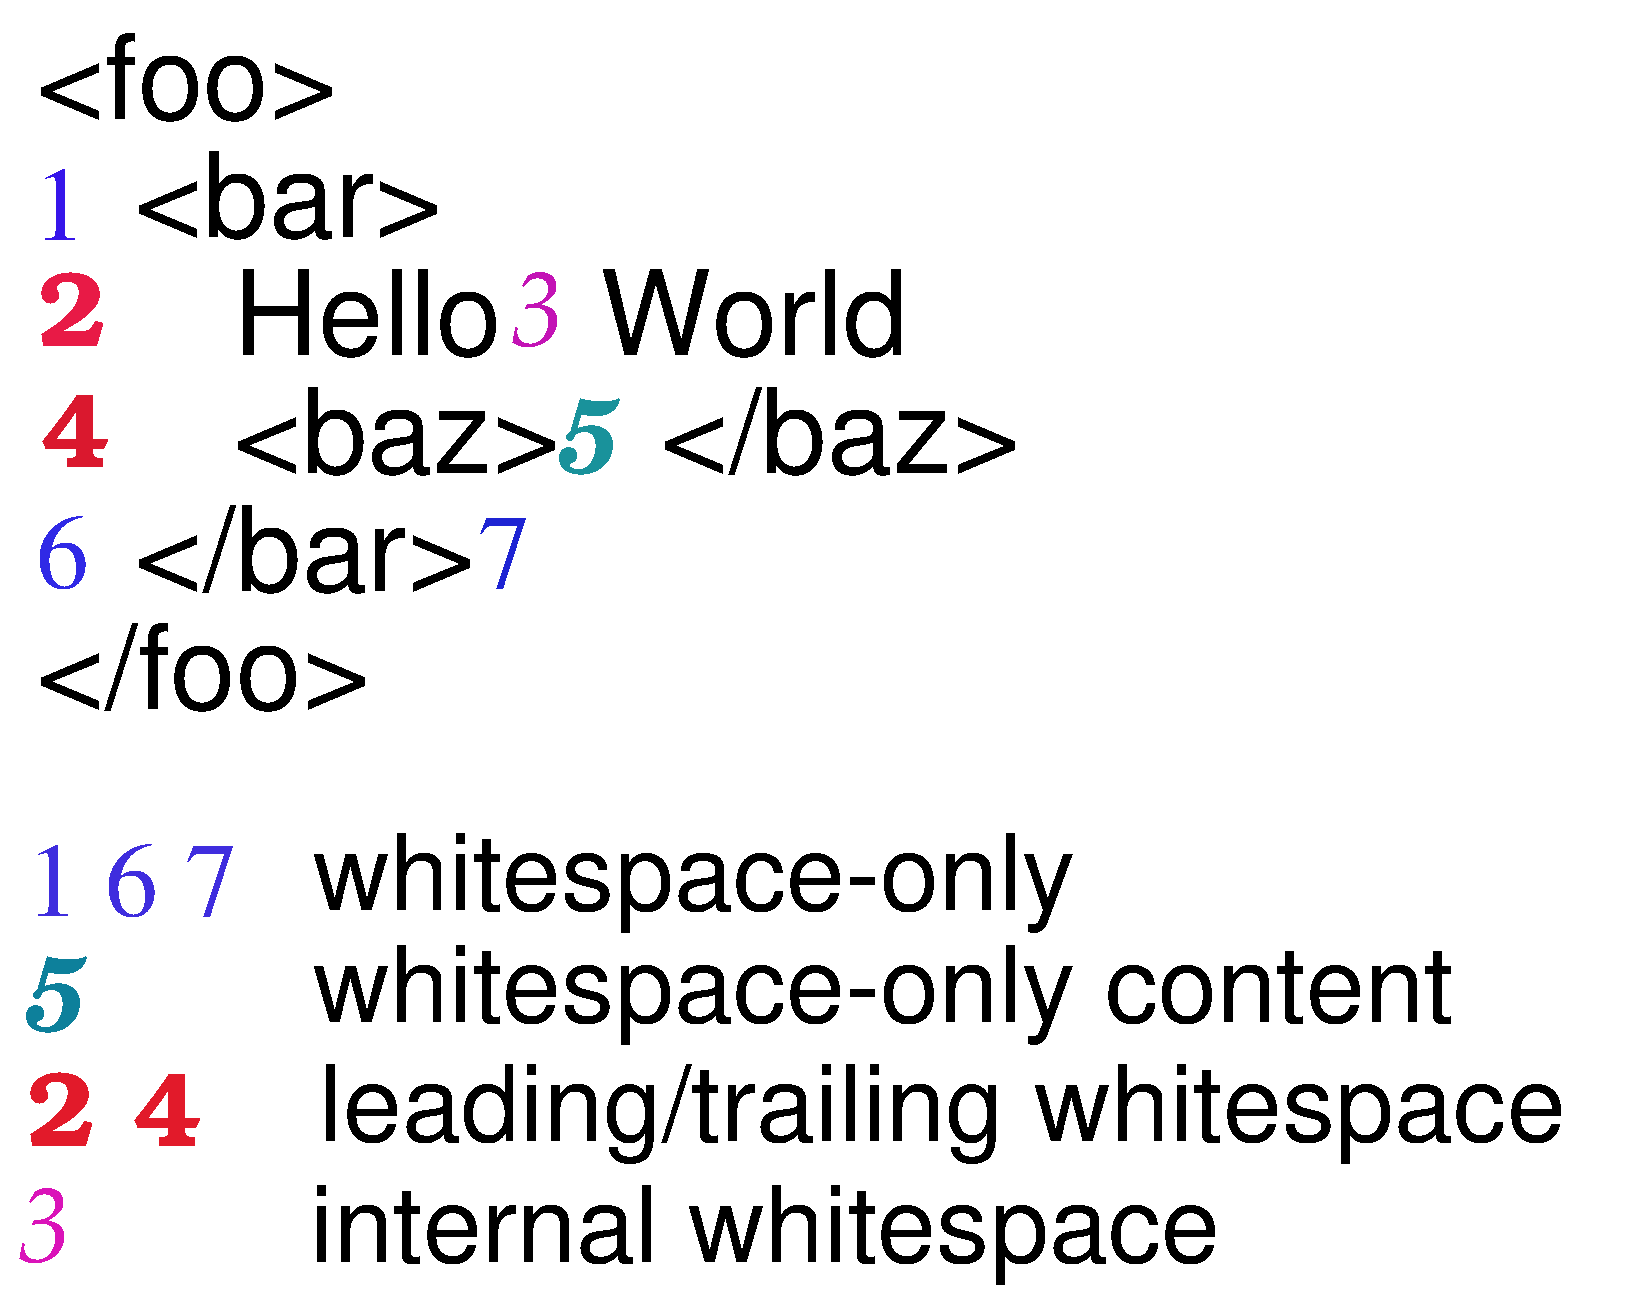
\includegraphics[height=1.5in]{etl-whitespace-rules.eps}
\caption{The various classes of whitespace nodes in XML. \label{fig-ws-rules}}
\end{centering}
\end{figure}

ETL permits fine-grained control over the whitespace that will be
generated via two orthogonal special attributes that are allowed on
every XML element in source ETL documents: \smtexttt{@bl:space-nodes}
and \smtexttt{@bl:text-nodes}.  These attributes are inherited by
contained (i.e., children) elements and their contents unless
overridden.  They control the various classes of whitespace
illustrated in \figref{ws-rules} as follows.

\begin{itemize}
\item \smtexttt{@bl:space-nodes} controls whitespace-only (and
      whitespace-only content) nodes (1, 5, 6, and 7 in the figure).
\item \smtexttt{@bl:text-nodes} controls leading/internal/trailing whitespace of
      text nodes (2, 3, and 4 in the figure).
\end{itemize}

The allowed settings for \smtexttt{@bl:space-nodes} are:

\begin{description}
  
\item[\smtexttt{preserve}] Leave the whitespace unchanged
      
\item[\smtexttt{compact}] Replace sequences of 1 or more
      whitespace characters with a single space (0x20)
      
\item[\smtexttt{strip}] Eliminate the whitespace entirely

\item[\smtexttt{normalize}] Strip whitespace nodes that contain only
newline (0x0A) characters entirely; replace sequences of 1 or more
whitespace characters that include a space or a tab with a single
space (0x20)

\end{description}

In addition to the above, \smtexttt{@bl:text-nodes} permits asymmetric
handling of the left and right sides of the text nodes via values
\smtexttt{compact-(left|right)} and \smtexttt{trim-(left|right)}. 
Importantly, all of these whitespace rules are statically-scoped:
a called template does not inherit the attributes from the calling
templates attribute annotations.

\subsection{Literal markup}
\label{ssec-literal-markup}

\gjb{write this section!}

** conditional tags

** at:*

** ?foo syntax, explain the tradeoff here

** building URIs

\subsection{Control constructs}
\label{ssec-control}

\gjb{write this section!}

** bl:if, with lots of slots to avoid a domain specific language
(ignore the fact that we have gotos and labels)

** bl:choose/bl:when/bl:otherwise

** bl:try/bl:catch/bl:finally

\subsection{Custom tags}
\label{ssec-custom-tags}

\gjb{write this section!}

** mention Scheme hygienic macro system; similar to that, except uses
XSLT for rewrite rules.

** Cite Simonyi, et al.'s ``Transformation in Intentional Programming''

** iterate until no more custom tags to expand

** expand before or after WS handling



\begin{figure}[tb]
\begin{centering}
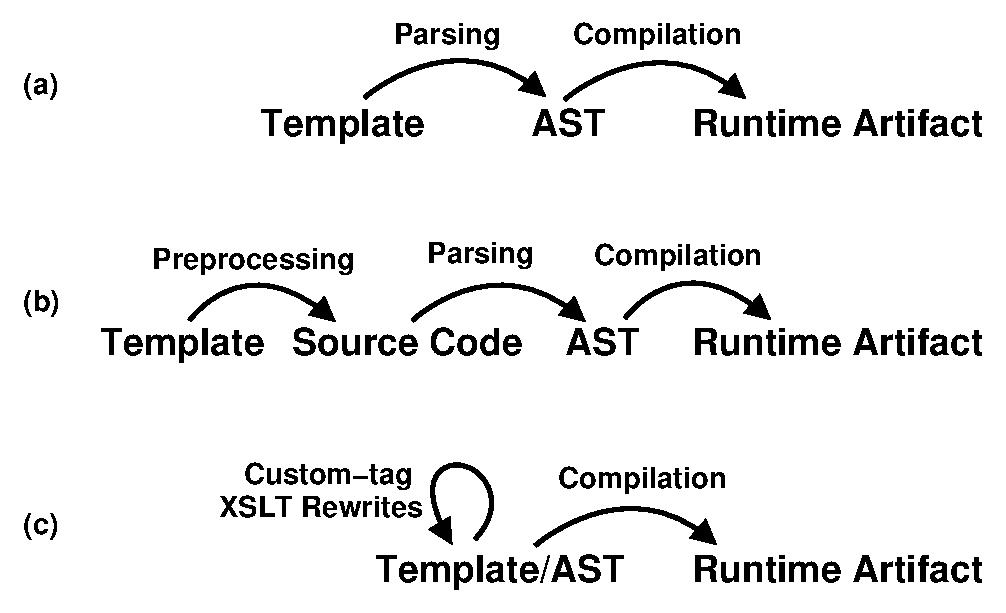
\includegraphics[width=1\linewidth]{processing-stages-simple.eps}
\caption{Overview of various templating languages pre-execution
processing.  The pipeline (a) illustrates a mod\_perl-like system where
the template is parsed and then byte-compiled into the runtime
artifact, while (b) shows a JSP-like preprocessing system where the
template is first converted into textual source code which then is
parsed and compiled.  ETL's use of XML (c) allows the web developer to
manipulate and analyze the AST thus simplifying the system.
\label{fig-processing-stages}}
\end{centering}
\end{figure}


\subsection{Invoking applications}

** HTTP GET/POST

** ws-call

** accessing abstract data model keyed off of content source name
(this is kevxml -- maybe call it kxmlinclude?)


%%% 
\section{Benefits of ETL}
\label{sec-benefits}

ETL has an integrated development environment that was very
easy to build by leveraging the XSD schema that defines the language
(\figref{homesite-screenshot}).

* two things: reduce expressiveness and use XML representation

** development environment completion
** validation for deep checking before deployment
** pretty-printing 
** source->source transformation 
** new abstractions 
** reduce app-level security holes (ref. scott \& sharp)
** call graph extraction
** provable termination (bounded recursion and only data-driven iteration over finite data structures)
** simpler: no need to mix programming paradigms, no need to learn a general purpose programming language: XML + web services *IS* your world

\begin{figure}[tb]
\begin{centering}
\hspace*{-0.05\linewidth}\includegraphics[width=1.1\linewidth]{homesite-screenshot.eps}
\caption{A screenshot of the integrated development environment based
on Homesite.  By using custom tag information generated automatically
from the XSD schema for ETL, the environment supports automatic
completion of names of elements and their valid attributes.  Help
information extracted from the server codebase is also readily
available in the IDE\@.
\label{fig-homesite-screenshot}}
\end{centering}
\end{figure}



%% This was generated using:
%% ~/tigerprawns/etl-interpreter/tools/templates-for-url.pl -r edges-ftr_fast.htm -A "http://stagingetl2/info/ftr_fast.htm"
%%  dot -Tgif edges-ftr_fast.htm > ftr_fast-call-graph.gif
%% and then converting the .GIF into .EPS using XV
\begin{figure*}[bt]
\begin{centering}
\includegraphics[width=\linewidth]{ftr_fast-call-graph.eps}
\caption{Call-graph of templates possibly used in generating an HTML
page footer.  The extraction of the call-graph was done using
server-side XPath expressions and a simple Perl script. \label{fig-call-graph}}
\end{centering}
\end{figure*}


%%% 
\section{Implementation \& experience}
\label{sec-implementation}

A byte-code compiler and runtime for the Extensible Templating Language is
an integral part of InfoSpace's ETL Server.  ETLS is architected as an
ISAPI extension to Microsoft's IIS and could be easily ported to any
web server that exposes a similar Extension Control Block interface.
IIS is used to manage the raw socket connections and many HTTP
protocol details, but ETLS generates the response for all incoming
requests (including static files which are still subject to template
selection rules).

** ETLS, its goals, backward-compatibility needs

** Server principles
*** be an appliance box: everything via HTTP
*** support MS management interfaces (mmc, win* service)

ETL has a debugger (\figref{debugger-screenshot}).  Solve fundamental
problem of needing to have stderr output for web development.

% ?etl-* parameters
% security
% inspadmin:* directives & the startup configuration file

%%% MAYBE MOVE THIS TO THE BENEFITS SECTION??
\begin{figure}[tb]
\begin{centering}
\hspace*{-0.03\linewidth}\includegraphics[width=1.1\linewidth]{debugger-screenshot.eps}
\caption{A screenshot of the debugger.
\label{fig-debugger-screenshot}}
\end{centering}
\end{figure}


\begin{figure}[tb]
\begin{centering}
\hspace*{-0.05\linewidth}\includegraphics[width=1.1\linewidth]{etls-admin-screenshot.eps}
\caption{The ETL Server's administration pages.
\label{fig-etls-admin}}
\end{centering}
\end{figure}



\begin{figure}[htbp]
\begin{verbatim}
Template `books.html.etl' has 0 errors.
0 template('books.html.etl') {
1  set_simple(#xml/books := '...')
2  #nocmd('<html>','</html>') {
3   #nocmd('<table>','</table>') {
4    for-each(#xml/books/book) {
5     #nocmd('<tr>','</tr>') {
6      #nocmd('<td>','</td>') {
7       get(@author)
       } // #nocmd('<td>','</td>')
8      #nocmd('<td>','</td>') {
9       get(@title)
       } // #nocmd('<td>','</td>')
      } // #nocmd('<tr>','</tr>')
     } // for-each(#xml/books 'book')
    } // #nocmd('<table>','</table>')
   } // #nocmd('<html>','</html>')
  } // template('books.html.etl')
\end{verbatim}
\caption{A server-generated decompilation of the internal representation
of the ETL template from \figref{etl-books}.  The nesting of elements
is preserved, but the byte-codes have been linearized for performance.
\label{fig-etl-decompile}}
\end{figure}


%%% 
\section{Related work}
\label{sec-related-work}

\gjb{write these up nicely}

JavaML -- key observation is that folks are already writing XML when
doing markup templating, so it is a natural place to apply the
benefits of an XML-based program representation.  Cite Zou \&
Kontogiannis; Power \& Malloy; Maletic, Collard, \& Marcus; Schonger,
Pulvermiller \& Sarstedt; 

XSLT -- declarative and that confuses folks.  Plus too limited in
terms of ability to interact with external components -- you end up
having to use a mix of XSLT and a scripting language with all the
problems that entails.  Also, no streaming mechanism.

LAML -- the dual of ETL -- took markup and embedded it in Scheme,
whereas ETL takes only the most critical programming constructs and
embeds them in XML.  Mention S-exp and XML similarity.

BigWig -- similar goals, but take a general purpose programming
language and extend it with a first class markup fragment type with
gaps that can be plugged.  They do lattice-theoretic iterative
data-flow analyses, ETL focusses on practical aspects of limiting
common mistakes:  it'd be interesting to apply the data flow analyses
to ETL to make it provably generate correct markup, but that wasn't an
a priori goal.

Modeling HTML in Haskell \& Typed representation for HTML \& XML in Haskell


%%% 
\section{Conclusions \& future work}
\label{sec-conclusion}

* Restate contribution, stress in actual use


** XML infoset and non-infoset artifacts
*** a bit problematic for source->source and for representing literal markup
** alternate syntax (a la stylescript) for other purposes
*** importantly, has an implied XML data model (e.g., can be algorithmically turned into the other syntax)
** math and conditionals
** generalized content-slot
** improvements to XSD to enable better validation
*** e.g., either/or attributes for slots
*** custom tag element definitions
** levels of strictness
** data flow analyses to infer needs for xmlencoding of variable values
** taint tracking of input variables
** better warning/error reporting in terms of the pre-macro-transformed source template

** Considering domain specific languages for bl:calc/@expr and bl:if/@test

\section{Acknowledgments}
\label{sec-ack}
This research is supported by InfoSpace and its advanced server
development group.  I thank Russ Arun and Steve Newman for their early
recognition of the value of this approach and their support.  ETL
itself was designed in collaboration with Abhishek Parmar and is
influenced by the legacy language of its predecessor web server which
was implemented by Jean-Remy Facq.  The ETL Server was built by the
author along with Abhishek Parmar, Venkatesh Juryala, Sridhar Koneru,
Mark Sandori, Michael Harrison, Kris Bradley, Angela Plyler, Sunil
Thomas, and Howard Zhao.  Testing of ETLS was ably performed by Zine
Rif, Sriram Krishnan, Michael Schaffer, Shavkat Azimov, Jeff Wells,
Ilian Georgeiw, and Russell Ashmun, and credit goes to Antonio
Casacuberta for continued support of the server group.  I also thank
Jeff Torgerson, Matthew Benedict, Vasanth Cattamanchi and all of the
InfoSpace web developers for their input and contributions to
the system. ETLS is a trademark of InfoSpace, Inc.


\bibliographystyle{abbrv}
\bibliography{etl-www2003}  % sigproc.bib is the name of the Bibliography in this case

%
%\balancecolumns
%\appendix
%Appendix A
%\section{}
%\balancecolumns % GM July 2000

\end{document}
